% =============================================================================
%  Capítulo 2: Métodos basados en gradiente
%  Basado en:
%    Steven L. Brunton, "Optimization: A Bootcamp for Machine Learning,
%    Inverse Problems, and Control", Cambridge University Press, 2026.
%    Capítulo 2, secciones 2.1--2.7 (pp. 47-88).
%
%  Contenido verificado del capítulo:
%    2.1 Gradient Descent
%    2.2 Momentum Methods
%    2.3 Stochastic Gradient Descent and ADAM
%    2.4 Newton's Method
%    2.5 Line Search
%    2.6 Quasi-Newton Methods and BFGS
%    2.7 Gradient Vector Calculus Identities
%
%  Compilar:  make
% =============================================================================

\documentclass[10pt,aspectratio=169]{beamer}

% --- Idioma y codificación ---------------------------------------------------
\usepackage[utf8]{inputenc}
\usepackage[T1]{fontenc}
\usepackage[spanish]{babel}

% --- Matemáticas -------------------------------------------------------------
\usepackage{amsmath,amssymb,mathtools}

% --- Tablas y diseño ---------------------------------------------------------
\usepackage{booktabs}
\usepackage{tabularx}
\usepackage{array}
\usepackage{lmodern}
\usepackage{microtype}

% --- Colores -----------------------------------------------------------------
\definecolor{unah}{RGB}{0,82,155}
\definecolor{acento}{RGB}{0,135,110}

\setbeamercolor{structure}{fg=unah}
\setbeamercolor{frametitle}{fg=unah}
\setbeamercolor{itemize item}{fg=acento}
\setbeamercolor{itemize subitem}{fg=unah}
\setbeamertemplate{itemize item}{\color{acento}\scriptsize$\blacktriangleright$}
\setbeamertemplate{itemize subitem}{\color{unah}\scriptsize$\bullet$}

% --- Plantillas --------------------------------------------------------------
\setbeamertemplate{navigation symbols}{}
\setbeamertemplate{footline}[frame number]

% --- Fuente de las figuras ---------------------------------------------------
\newcommand{\fuente}{\vfill{\scriptsize\color{gray}Brunton, \emph{Optimization Bootcamp}, Cap.~2}}

% --- Espacio reservado para figuras (sin imagenes por ahora) -----------------
% Uso: \figura{Descripcion del contenido}{0.85\textwidth}{2.2cm}
\newcommand{\figura}[3]{%
  \begin{center}
    \fbox{\parbox[c][#3][c]{#2}{%
      \centering\small\color{gray}
      \textbf{Espacio reservado para figura}\\[3pt]
      \footnotesize #1}}%
  \end{center}%
}

\title{Cap. 2: Métodos Iterativos de Gradiente}

% =============================================================================
\begin{document}
% =============================================================================

% --- Portada -----------------------------------------------------------------
\begin{frame}
  \titlepage
\end{frame}

% --- Esquema -----------------------------------------------------------------
\begin{frame}{Esquema de la presentación}
  \tableofcontents
\end{frame}

% =============================================================================
\section{¿Por qué métodos iterativos?}
% =============================================================================

\begin{frame}{El problema central}
  \small
  \begin{itemize}
    \item Mínimo local de $f$ suave y sin restricciones:
      \[
        \nabla f(x^\star)=0, \qquad \nabla^2 f(x^\star)\succeq 0.
      \]
    \item En general \emph{no} se resuelve $\nabla f(x)=0$ de forma explícita.
    \item Se busca una sucesión $x_{k+1}=F(x_k)$ tal que
      \[
        f(x_0)\ge f(x_1)\ge \cdots \ge f(x_k) \to f(x^\star).
      \]
    \item Algoritmo ideal: rápido, monotono y de bajo coste por iteración.
  \end{itemize}
  \begin{alertblock}{Advertencia}
    El resultado solo es óptimo local, salvo que el problema sea convexo.
    En problemas no convexos la inicialización $x_0$ decide a qué mínimo se llega.
  \end{alertblock}
\end{frame}

\begin{frame}{Dos familias}
  \small
  \begin{columns}[T,onlytextwidth]
    \begin{column}{.48\textwidth}
      \textbf{Métodos de primer orden}
      \begin{itemize}
        \item Usan $\nabla f$.
        \item Aproximación lineal de $f$.
        \item Escala a sistemas muy grandes.
        \item Base del aprendizaje automático.
        \item Ej.: gradiente, momento, \emph{SGD}, ADAM.
      \end{itemize}
    \end{column}
    \begin{column}{.48\textwidth}
      \textbf{Métodos de segundo orden}
      \begin{itemize}
        \item Usan $\nabla^2 f$ (Hessiano).
        \item Aproximación cuadrática de $f$.
        \item Menos iteraciones.
        \item Mayor coste y memoria.
        \item Ej.: Newton, \emph{quasi}-Newton, BFGS.
      \end{itemize}
    \end{column}
  \end{columns}
  \vfill
  {\scriptsize\color{gray}
    Ventaja común: se asume muy poca estructura, solo la existencia de derivadas.}
\end{frame}

% =============================================================================
\section{Descenso de gradiente}
% =============================================================================

\begin{frame}{El algoritmo}
  \small
  \[
    \boxed{\;x_{k+1}=x_k-\gamma\,\nabla f(x_k)\;}
  \]
  \begin{itemize}
    \item $-\nabla f(x_k)$ es la dirección de máximo descenso local.
    \item $\gamma>0$ es el tamaño de paso o \emph{learning rate}.
    \item Se apoya en la aproximación de Taylor de primer orden:
      \[
        f(x_k+\Delta x)\approx f(x_k)+\nabla f(x_k)^{T}\Delta x.
      \]
    \item Cerca del mínimo el gradiente se hace pequeño y los pasos se acortan solos.
    \item En objetivos no convexos, cada punto cae en el mínimo local más cercano.
  \end{itemize}
  \fuente
\end{frame}

\begin{frame}{¿Cómo elegir el paso $\gamma$?}
  \small
  \begin{tabularx}{\textwidth}{@{}>{\bfseries}l X@{}}
    \toprule
    Criterio & Descripción \\
    \midrule
    Fijo & Simple; funciona bien si el Hessiano está bien condicionado. \\
    Armijo & Solo depende del gradiente y garantiza el descenso. \\
    Decreciente & $\gamma_k=\gamma_0/(1+\beta k)$; pasos grandes al inicio. \\
    Búsqueda lineal & Optimiza $\gamma$ en cada iteración (Sección 2.5). \\
    Momentum & Aporta inercia para cruzar regiones planas (Sección 2.2). \\
    Adaptativo & RMSProp y ADAM ajustan el paso con el historial. \\
    Programas & Decaimiento exponencial u otros horarios por etapas. \\
    \bottomrule
  \end{tabularx}
  \vfill
  {\scriptsize\color{gray}
    \textbf{Panel 2.1.} Búsqueda lineal:
    $\gamma_k=\arg\min_{\gamma>0}f(x_k-\gamma\nabla f(x_k))$;
    en la práctica se recorre $\gamma$ de forma iterativa.}
\end{frame}

\begin{frame}{Ejemplo cuadrático}
  \small
  \[
    f(x)=\tfrac12 x^{T}Ax, \qquad
    A=\begin{bmatrix}2&1\\1&3\end{bmatrix} \succ 0,
    \qquad x^\star=0.
  \]
  \begin{itemize}
    \item Problema de referencia: la solución se conoce de antemano.
    \item $\gamma=0.01$: convergencia lenta.
    \item $\gamma=0.1$: convergencia rápida y sin oscilaciones.
    \item $\gamma=0.543$: casi inestable, oscila alrededor del mínimo.
  \end{itemize}
  \begin{figure}
      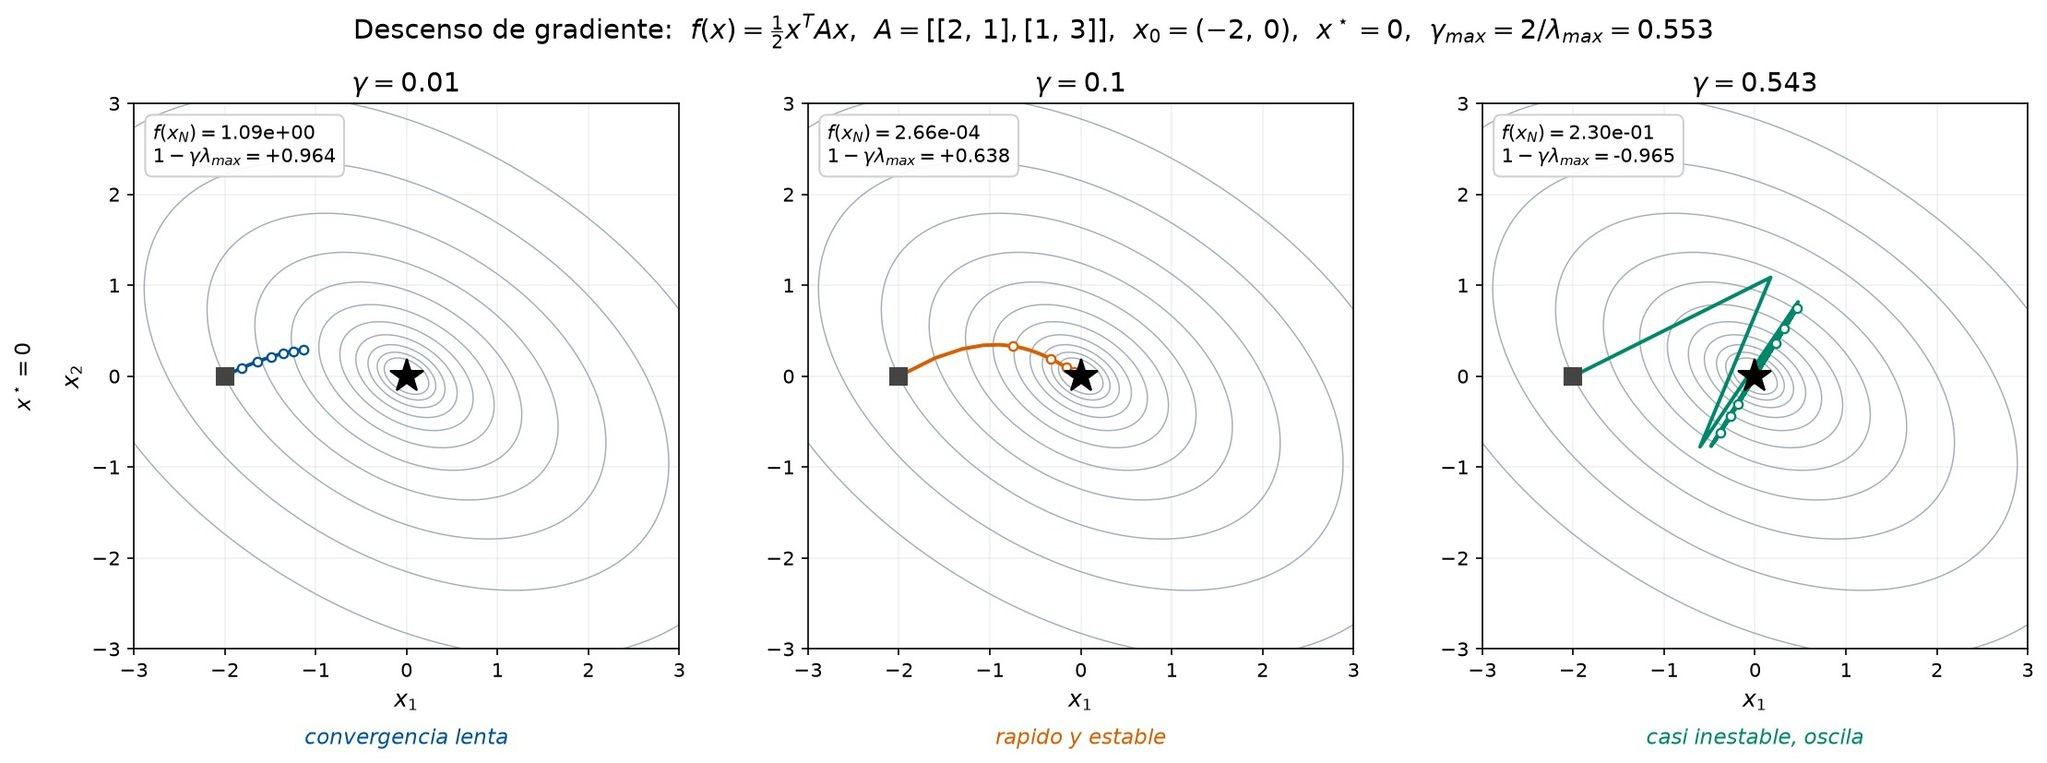
\includegraphics[width=0.6\textwidth]{images/step_size.jpg}
  \end{figure}
\end{frame}

\begin{frame}{Convergencia de gradiente}
  \small
  \textbf{Caso 1.} $f$ convexa y $\nabla f$ Lipschitz con constante $L$, con $\gamma=1/L$:
  \[
    f(x_k)-f(x^\star)\le\frac{L}{2k}\,\|x_0-x^\star\|^2
    \qquad\Longrightarrow\qquad \mathcal{O}(1/k).
  \]
  \textbf{Caso 2.} $f$ $\mu$-fuerte convexa:
  \[
    f(y)\ge f(x)+\nabla f(x)^{T}(y-x)+\tfrac{\mu}{2}\|y-x\|^2,
  \]
  \[
    f(x_k)-f(x^\star)\le\frac{L}{2}
      \left(1-\frac{\mu}{L}\right)^{k}\|x_0-x^\star\|^2.
  \]
  \begin{itemize}
    \item Para $f(x)=\tfrac12 x^{T}Ax$ se cumple $\mu=\lambda_{\min}(A)$.
    \item La fuerte convexidad se reutiliza en la envoltura de Moreau (Sección 5.1).
  \end{itemize}
\end{frame}

\begin{frame}{Flujo de gradiente}
  \small
  Considérese la ecuación diferencial
  \[
    \dot x(t)=-\nabla f\big(x(t)\big).
  \]
  El campo $-\nabla f$ es un \emph{gradient flow}: conservativo, irrotacional e
  incompresible si $\nabla^2f=0$. El paso de Euler hacia adelante es
  \[
    x_{k+1}=x_k+\Delta t\,v(x_k),
  \]
  y al tomar $\Delta t=\gamma$ se recupera exactamente el descenso de gradiente.
  \begin{block}{Consecuencia}
    Un esquema numérico mejor para el mismo flujo, como Runge--Kutta de orden superior,
    produce un algoritmo de descenso distinto (ejercicios 2.7 y 2.8).
  \end{block}
  \vfill
  {\scriptsize\color{gray}Panel 2.2}
\end{frame}

\begin{frame}{Estabilidad en el caso cuadrático}
  \small
  \[
    f(x)=\tfrac12x^{T}Ax+b^{T}x+c,\qquad \nabla f(x)=Ax+b.
  \]
  \[
    x_{k+1}=x_k-\gamma(Ax_k+b)=(I-\gamma A)x_k-\gamma b.
  \]
  \begin{itemize}
    \item El factor iterativo es $I-\gamma A$, con autovalores $1-\gamma\lambda_j$.
    \item $A$ simétrica: $\nabla^2f=A$. Si $A$ no lo es,
      $\nabla f=\tfrac12(A+A^{T})x+b$ y $\nabla^2f=\tfrac12(A+A^{T})$.
    \item Estabilidad: $|1-\gamma\lambda_j|<1$ para todo $j$.
    \item De ahí
      \[
        \boxed{\,0<\gamma<\gamma_{\max}=\frac{2}{\lambda_{\max}}\,}.
      \]
  \end{itemize}
\end{frame}

\begin{frame}{Paso óptimo}
  \small
  La tasa la fija el radio espectral $\rho(I-\gamma A)=\max_j|1-\gamma\lambda_j|$.
  Los autovalores son simétricos respecto de $1-\gamma\lambda_{\mathrm{mid}}$, con
  $\lambda_{\mathrm{mid}}=(\lambda_{\min}+\lambda_{\max})/2$.
  El mínimo se alcanza al distribuirlos simétricamente respecto del origen:
  \[
    1-\gamma^{\star}\lambda_{\min}=-(1-\gamma^{\star}\lambda_{\max}),
  \]
  \[
    \boxed{\;\gamma^{\star}=\frac{2}{\lambda_{\min}+\lambda_{\max}}\;},
    \qquad
    \boxed{\;\rho=\frac{\lambda_{\max}-\lambda_{\min}}{\lambda_{\min}+\lambda_{\max}}\;}.
  \]
  \begin{itemize}
    \item $\rho$ es la contracción peor caso por iteración.
    \item Gran dispersión de autovalores $\Rightarrow$ convergencia lenta.
  \end{itemize}
\end{frame}

\begin{frame}{¿Por qué iterar si $Ax=b$?}
  \small
  Aunque $x^\star=-A^{-1}b$ se pueda calcular, el descenso de gradiente conviene cuando
  la inversa es intratable:
  \begin{itemize}
    \item \textbf{$A$ grande:} con $n$ en millones o miles de millones, $A^{-1}$ ni siquiera
      cabe en memoria; el producto $Ax$ sí puede estar disponible.
    \item \textbf{$A$ dispersa:} común en física (mecánica de fluidos: difusión y convección
      son interacciones locales); los métodos iterativos ganan.
    \item \textbf{$A$ mal condicionada:} la inversión directa es inexacta; se usan
      precondicionadores y descenso iterativo.
  \end{itemize}
  \fuente
\end{frame}

% =============================================================================
\section{Métodos con momento}
% =============================================================================


\begin{frame}{Métodos de Momentum}
    \framesubtitle{También conocido como Heavy-Ball}
    Para reducir el problema del zig-zag, agregamos el un término a la iteración:
  \small
  \[
    \boxed{\;x_{k+1}=x_k-\gamma\nabla f(x_k)+\beta\,(x_k-x_{k-1})\;}
  \]
  o, introduciendo la velocidad $v_k=x_k-x_{k-1}$:
  \[
    v_{k+1}=\beta v_k-\gamma\nabla f(x_k),
    \qquad
    x_{k+1}=x_k+v_{k+1}.
  \]
  \begin{itemize}
    \item Nuevo hiperparámetro $\beta\in[0,1)$: tasa de decaimiento de la velocidad.
    \item $v_k$ es una suma descontada exponencialmente de gradientes previos.
    \item $\beta=0$ recupera el descenso de gradiente simple.
  \end{itemize}
  \fuente
\end{frame}

\begin{frame}{Heavy ball como sistema mecánico}
  \small
  La iteración surge de la EDO de segundo orden con fricción
  \[
    m\ddot x(t)=-\nabla f\big(x(t)\big)-\delta\,\dot x(t).
  \]
  Con diferencias centradas para $\ddot x$ y Euler para $\dot x$, paso $\Delta t$:
  \[
    \gamma=\frac{\Delta t^{2}}{m+\delta\,\Delta t},
    \qquad
    \beta=\frac{m}{m+\delta\,\Delta t}.
  \]
  \begin{itemize}
    \item $m$ es la masa (inercia) y $\delta$ el coeficiente de fricción.
    \item Si $\delta=0$: $\beta=1$, sin pérdida de momento.
    \item Relación explícita entre los hiperparámetros y la dinámica física.
  \end{itemize}
  \vfill
  {\scriptsize\color{gray}Panel 2.3}
\end{frame}

\begin{frame}{Nesterov: mirar antes de bajar}
  \small
  \[
    \boxed{
      \begin{aligned}
      y_k&=x_k+\beta v_k &&\text{(punto anticipado)}\\
      x_{k+1}&=y_k-\gamma\nabla f(y_k)
      \end{aligned}}
  \]
  \begin{itemize}
    \item Único cambio respecto a heavy ball: el gradiente se evalúa en $y_k$, no en $x_k$.
    \item Equivale a un esquema tipo Runge--Kutta.
    \item Sutskever: NAG invierte el orden de momentum y descenso.
    \item Ventaja: la dirección ya incorpora la inercia, así no se pierde
      velocidad al llegar a una región plana.
  \end{itemize}
\end{frame}

\begin{frame}{Convergencia de Nesterov}
  \small
  \textbf{$f$ convexa, $\nabla f$ Lipschitz con constante $L$:}
  \[
    f(x_k)-f(x^\star)\le\frac{2L}{(k+1)^2}\,\|x_0-x^\star\|^2
    \qquad\Longrightarrow\qquad \mathcal{O}(1/k^{2}).
  \]
  \textbf{$f$ $\mu$-fuerte convexa:}
  \[
    f(x_k)-f(x^\star)\le
      2\left(1-\sqrt{\tfrac{\mu}{L}}\right)^{k}
      \big[f(x_0)-f(x^\star)\big].
  \]
  \begin{itemize}
    \item De $\mathcal{O}(1/k)$ a $\mathcal{O}(1/k^{2})$: gran mejora.
    \item Caso fuerte convexo: decaimiento geométrico, es decir lineal.
  \end{itemize}
\end{frame}

\begin{frame}{Nesterov como EDO}
  \small
  \[
    \ddot x(t)+\frac{3}{t}\dot x(t)+\nabla f\big(x(t)\big)=0,
  \qquad x(0)=x_0,\quad \dot x(0)=0.
  \]
  \begin{itemize}
    \item El límite continuo de NAG es esta EDO de segundo orden.
    \item El tiempo se relaciona con el paso por $t\approx\sqrt{k\gamma}$,
      con $\gamma\le 1/L$.
    \item El término $3/t$ es el que aporta la ganancia de orden dos.
  \end{itemize}
\end{frame}

\begin{frame}{AdaGrad y RMSProp}
  \small
  \textbf{AdaGrad:} acumula los cuadrados del gradiente, coordenada a coordenada:
  \[
    r_k=r_{k-1}+g_k^{\odot 2},
    \qquad
    x_{k+1}=x_k-\gamma\,\frac{g_k}{\sqrt{r_{k+1}}+\epsilon}.
  \]
  \begin{itemize}
    \item Cada coordenada recibe un paso propio según su historial.
    \item Problema: $r_k$ sólo crece, así que el paso se apaga con el tiempo.
  \end{itemize}
  \textbf{RMSProp:} introduce un factor de decaimiento:
  \[
    \boxed{\;r_{k+1}=\beta_2 r_k+(1-\beta_2)\,g_k^{\odot 2}\;}
  \]
  \begin{itemize}
    \item Media móvil exponencial de cuadrados: paso acotado y estable.
    \item Particularmente eficaz con problemas mal condicionados.
  \end{itemize}
\end{frame}

% =============================================================================
\section{SGD y ADAM}
% =============================================================================

\begin{frame}{Mínimos cuadrados como ajuste}
  \small
  Dados $N$ pares $(x_j,y_j)$, se buscan los parámetros $\theta$ que ajustan la función
  $f_\theta$:
  \[
    \min_{\theta}\;\sum_{j=1}^{N}\big\|f_\theta(x_j)-y_j\big\|^{2}.
  \]
  La función de pérdida es $L(x,y;\theta)=\|f_\theta(x)-y\|^{2}$, con gradiente
  \[
    \nabla L=2\,\nabla f_\theta^{T}\,(f_\theta(x)-y).
  \]
  \begin{itemize}
    \item Es un problema de mínimos cuadrados no lineal.
    \item $\nabla f_\theta$ se calcula analíticamente o por retropropagación.
    \item La retropropagación es la regla de la cadena aplicada capa a capa.
    \item Detalles en el Capítulo 10.
  \end{itemize}
\end{frame}

\begin{frame}{Descenso estocástico}
  \small
  En vez del gradiente sobre todo el conjunto, se usa un subconjunto aleatorio
  (un \emph{lote}):
  \[
    \hat\nabla L_k=\frac{1}{|B_k|}\sum_{j\in B_k}\nabla L(x_j,y_j;\theta),
    \qquad
    \boxed{\;\theta_{k+1}=\theta_k-\gamma\,\hat\nabla L_k\;}.
  \]
  \begin{itemize}
    \item La iteración es idéntica a la del gradiente clásico:
      la diferencia está escondida en el estimador del gradiente.
    \item Ventajas: velocidad, robustez al ruido, mejor exploración del
      paisaje y mejor generalización.
    \item Salida fácil: es la base de todas las variantes de momentum y
      de aprendizaje adaptativo.
    \item Nuevo hiperparámetro: el tamaño del lote.
  \end{itemize}
  \fuente
\end{frame}

\begin{frame}{Tamaño del lote}
  \small
  El gradiente completo y el SGD puro (lote de 1) son los extremos del mini-lote.
  \begin{itemize}
    \item Lote grande: menos ruido, pero más caro por paso.
    \item Lote pequeño: pasos más baratos y más rápidos, pero más ruido;
      con ruido fuerte conviene un lote mayor para amortiguarlo.
    \item En un ejemplo lineal, un lote de 10 equilibra convergencia y tiempo.
    \item Comparación típica: gradiente completo, mini-lote (50) y lote de 1.
      Los dos últimos convergen en muchas menos épocas.
  \end{itemize}
  \begin{alertblock}{Precaución}
    Una época de SGD con lote 1 son $N$ pasos individuales, no uno.
  \end{alertblock}
  \begin{figure}
  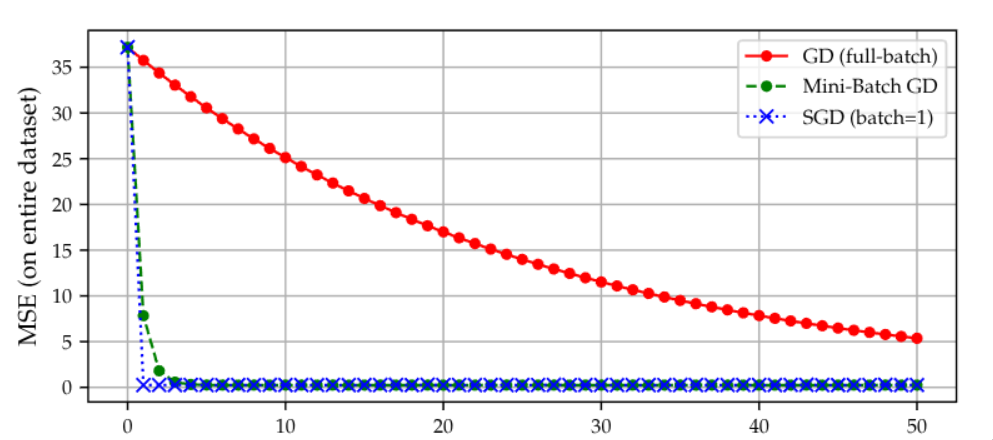
\includegraphics[width=0.5\textwidth]{images/sgd_conv.png}
  \end{figure}
\end{frame}

\begin{frame}{ADAM}
  \small
  Combina momentum (primer momento) con la escala adaptativa de RMSProp
  (segundo momento). Sea $g_k=\nabla f(x_k)$:
  \[
    m_k=\beta_1 m_{k-1}+(1-\beta_1)\,g_k,
    \qquad
    v_k=\beta_2 v_{k-1}+(1-\beta_2)\,g_k^{\odot 2},
  \]
  \[
    \hat m_k=\frac{m_k}{1-\beta_1^{k}},
    \qquad
    \hat v_k=\frac{v_k}{1-\beta_2^{k}},
  \]
  \[
    \boxed{\;x_{k+1}=x_k-\gamma\,
      \frac{\hat m_k}{\sqrt{\hat v_k}+\epsilon}\;}.
  \]
  \begin{itemize}
    \item Las correcciones $1-\beta^{k}$ unbiased estiman los momentos
      al principio, cuando están sesgados.
    \item El gradiente estocástico está implícito dentro de $\hat\nabla L$.
    \item Estándar de facto para entrenar redes neuronales:
      Su artículo original fue el más citado del mundo, en cualquier campo,
      durante una década completa.
  \end{itemize}
\end{frame}

% =============================================================================
\section{Método de Newton}
% =============================================================================

\begin{frame}{Aproximación cuadrática}
  \small
  En vez de la expansión lineal, se usa la de segundo orden:
  \[
    f(x)\approx f(x_k)+\nabla f(x_k)^{T}\Delta x
      +\tfrac12\Delta x^{T}\,H_k\,\Delta x,
    \qquad H_k=\nabla^{2}f(x_k).
  \]
  Derivando e igualando a cero,
  \[
    \nabla f(x_k)+H_k\Delta x=0
    \qquad\Longrightarrow\qquad
    \boxed{\;x_{k+1}=x_k-H_k^{-1}\nabla f(x_k)\;}.
  \]
  \begin{itemize}
    \item El Hessiano es simétrico (propiedad conmutativa de las derivadas mixtas).
    \item En una dimensión: $x_{k+1}=x_k-f'(x_k)/f''(x_k)$.
    \item Equivale al descenso de gradiente con paso $\gamma=1/H_k$.
  \end{itemize}
\end{frame}

\begin{frame}{Newton: convergencia y escalado}
  \small
  Si $f\in C^{2}$, $\nabla^{2}f$ es Lipschitz y $\nabla^{2}f(x^\star)$ es definido positivo:
  \[
    \lVert\epsilon_{k+1}\rVert\le C\,\lVert\epsilon_k\rVert^{2}.
  \]
  \begin{itemize}
    \item \textbf{Convergencia cuadrática:} los dígitos correctos casi se duplican
      en cada paso. Mucho más rápido que $\mathcal{O}(1/k^{2})$.
  \item \textbf{Costo:} $O(n^{3})$ para la inversa de $H$.
  \item Problema 1: el Hessiano puede ser casi-singular o demasiado caro.
    \item Problema 2: puede no ser definido positivo (máximo local o silla).
  \end{itemize}
  \begin{alertblock}{De ahí nacen los métodos \emph{quasi}-Newton.}
  \end{alertblock}
\end{frame}

\begin{frame}{Newton en la práctica}
  \small
  \begin{itemize}
    \item Nunca se invierte $H$ explícitamente: se resuelve $H_k p_k=-\nabla f(x_k)$.
    \item Lejos de $x_k$ el modelo cuadrático pierde calidad: se usa sólo
      para obtener la \emph{dirección} $p_k=H_k^{-1}\nabla f(x_k)$ y luego se
      hace una búsqueda lineal en esa dirección.
    \item Si $H_k$ no es definido positivo se amortigua:
      \[
        (H_k+\alpha I)p_k=-\nabla f(x_k),\qquad \alpha\ge0,
      \]
      y luego se busca el paso en la dirección $p_k$.
    \item Levenberg--Marquardt es el método clásico de Gauss--Newton amortiguado
      (Sección 4.7).
  \end{itemize}
  \begin{figure}
      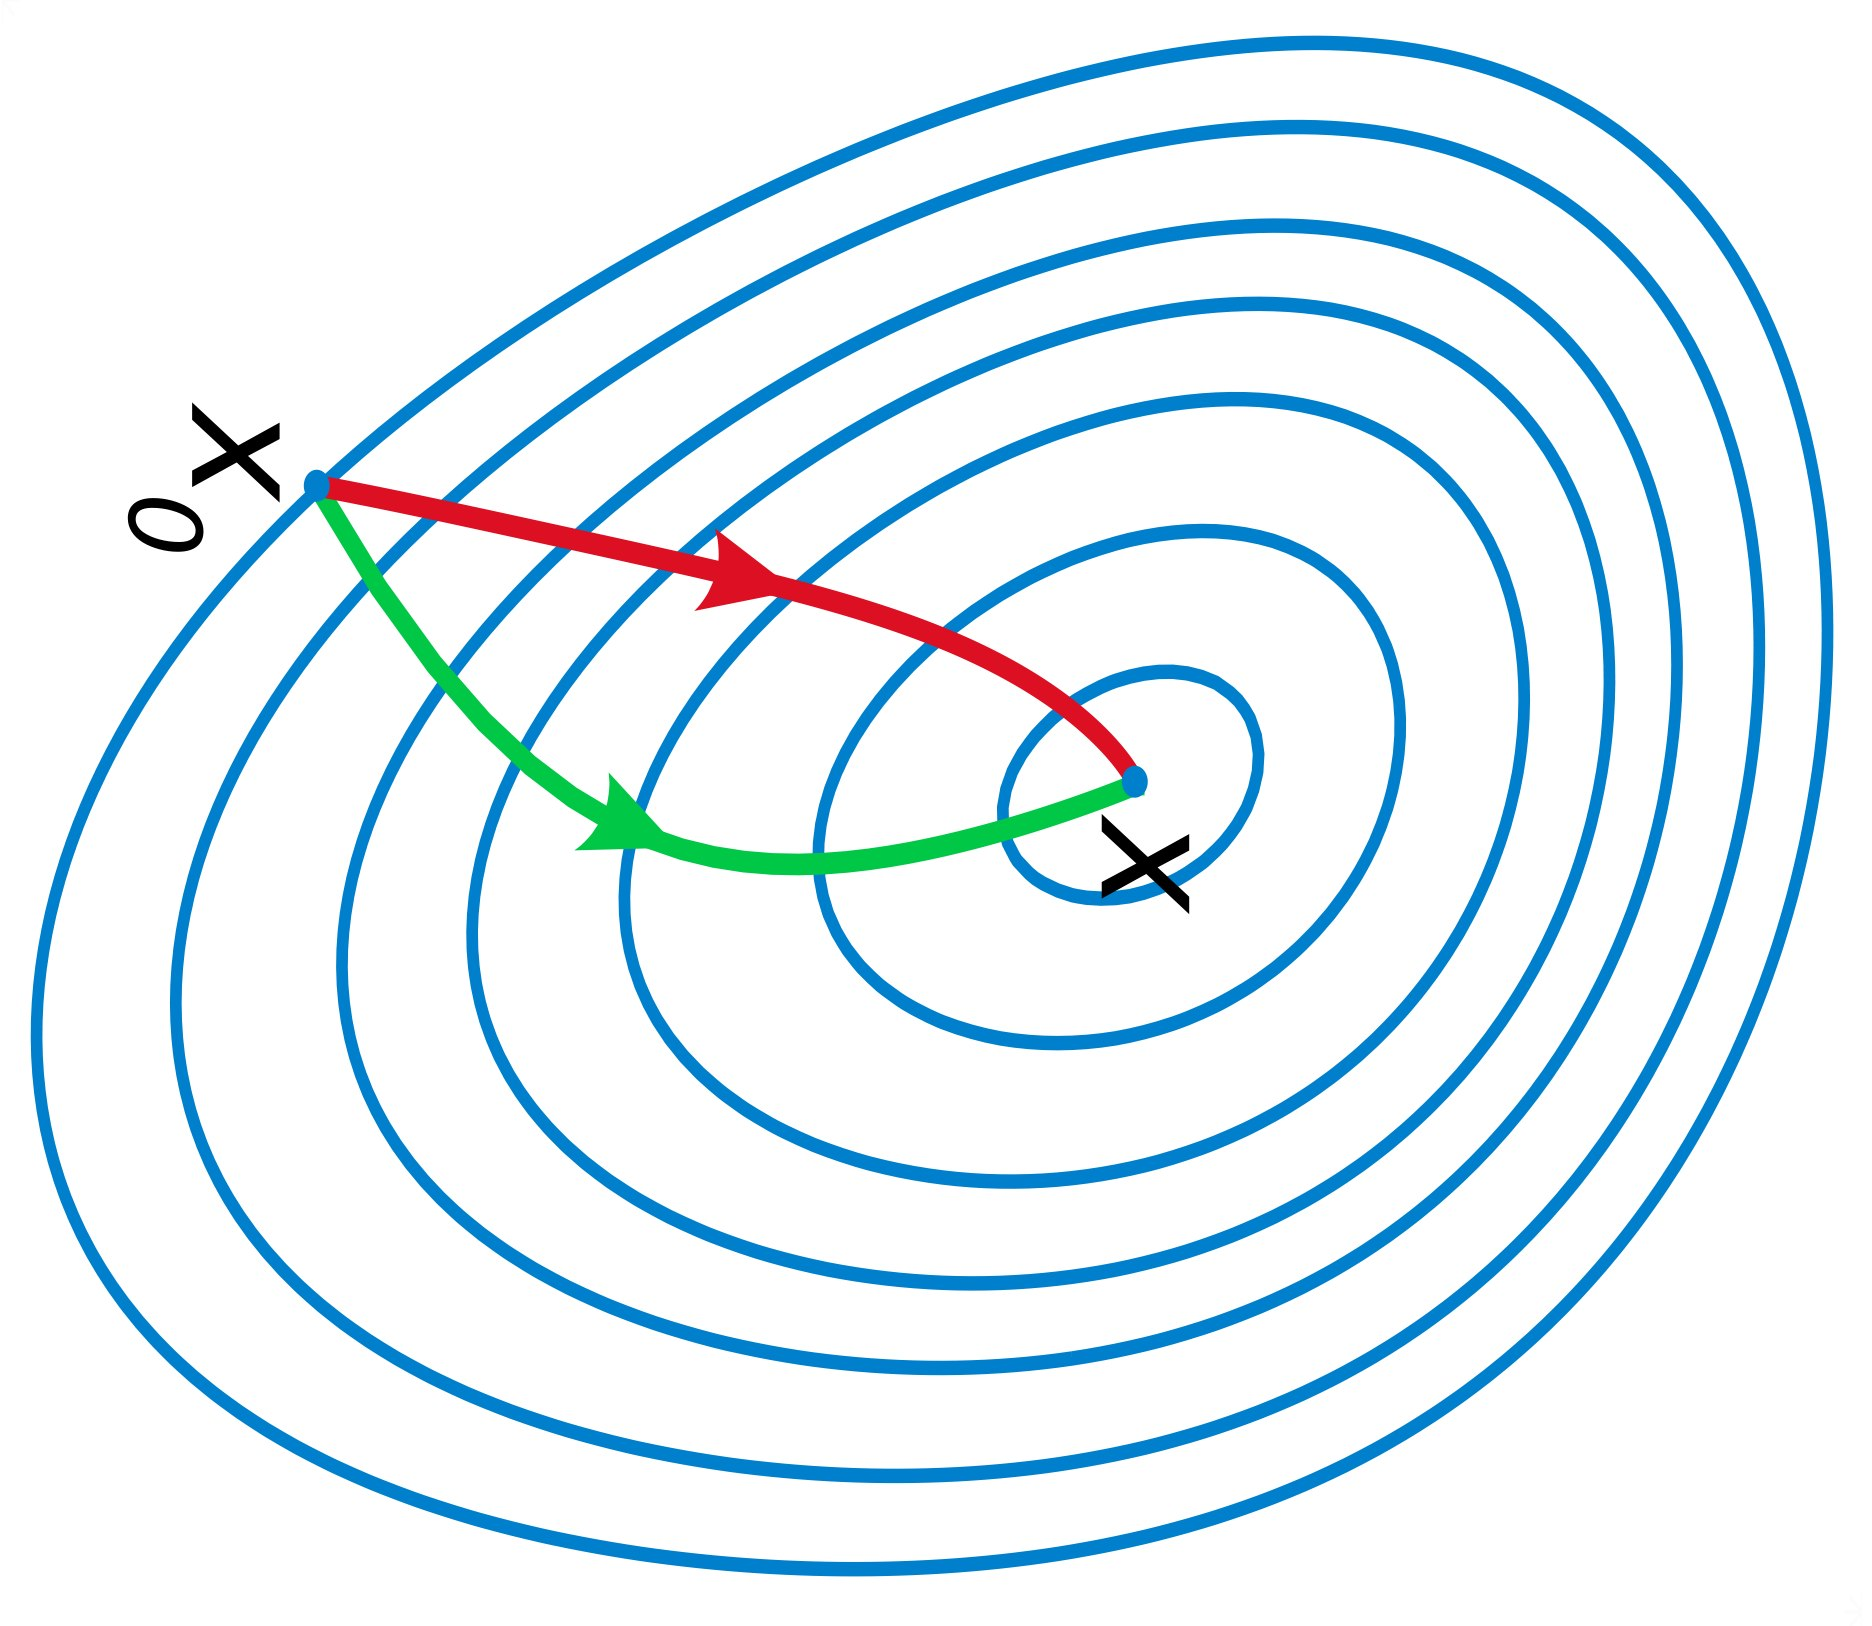
\includegraphics[width=0.3\textwidth]{images/comp_newton.jpg}
  \end{figure}
\end{frame}

% =============================================================================
\section{Búsqueda lineal}
% =============================================================================

\begin{frame}{Dirección y paso}
  \small
  Con una dirección de descenso $p_k$ y una iteración $x_{k+1}=x_k+\alpha_k p_k$:
  \begin{itemize}
    \item El \emph{algoritmo} elige la dirección $p_k$:
      gradiente, momentum o Newton.
    \item La \emph{búsqueda lineal} elige $\alpha_k>0$ de forma adaptativa.
    \item Búsqueda exacta: $\alpha_k=\arg\min_{\alpha>0}f(x_k+\alpha p_k)$.
      Casi nunca se usa, salvo en problemas cuadráticos.
    \item En la práctica se hace una búsqueda \emph{inexacta}: barrer $\alpha$.
  \end{itemize}
  \vfill
  \begin{block}{Por qué importa}
    Añade algunas evaluaciones de $f$ por iteración, pero reduce el número de
    iteraciones~\emph{un orden de magnitud} y aporta gran robustez.
    En métodos de segundo orden el sobrecoste es despreciable frente a calcular
    el Hessiano, así que se usa siempre.
  \end{block}
\end{frame}

\begin{frame}{Las tres familias}
  \small
  \begin{tabularx}{\textwidth}{@{}>{\bfseries}l X@{}}
    \toprule
    Criterio & Descripción \\
    \midrule
    Armijo & Disminución suficiente; robusto y fácil de implementar, aunque a
      veces demasiado conservador. \\
    Wolfe & Armijo más una condición de curvatura, que impide pasos demasiado
      pequeños. Es el usado en BFGS y L-BFGS. \\
    BB (Barzilai--Borwein) & Usa los dos últimos iterados para aproximar un paso
      \emph{quasi}-Newton; muy eficaz con problemas mal condicionados. \\
    \bottomrule
  \end{tabularx}
  \vfill
  \begin{block}{Regla práctica}
    Para gradiente completo: siempre Armijo, vuelve competitivo al gradiente
    con los métodos \emph{quasi}-Newton. Para Newton: esencial para la convergencia
    global. Con SGD la búsqueda lineal es difícil y poco habitual.
  \end{block}
\end{frame}

\begin{frame}{Armijo por retroceso}
  \small
  Con $d^TO\nabla f(x)<0$ (dirección de descenso), se busca $\alpha>0$ tal que
  \[
    \boxed{\;f(x+\alpha d)\le f(x)+c_1\,\alpha\,d^{T}\nabla f(x)\;},
    \qquad c_1\in(0,1).
  \]
  \begin{enumerate}
    \item Inicializar $\alpha\leftarrow\alpha_0$ (a menudo $\alpha_0=1$, o el tamaño
      del paso de Newton).
    \item Mientras no se cumpla: $\alpha\leftarrow\rho\,\alpha$ con $\rho\in(0,1)$
      (p. ej.\ $\rho=\tfrac12$), y volver a evaluar $f(x+\alpha d)$.
    \item Aceptar el primer $\alpha$ válido y actualizar $x\leftarrow x+\alpha d$.
  \end{enumerate}
  \begin{itemize}
    \item Valores habituales: $c_1\in[10^{-4},10^{-2}]$ y $\rho\in[0.1,0.8]$.
  \end{itemize}
\end{frame}

\begin{frame}{Condiciones de Wolfe}
  \small
  Además de la disminución suficiente, se exige una condición de curvatura:
  \[
    |d^{T}\nabla f(x+\alpha d)|\le c_2\,|d^{T}\nabla f(x)|,
    \qquad 0<c_1<c_2<1.
  \]
  \begin{enumerate}
    \item \textbf{Expansión:} se dan pasos de tamaño $\Delta x$ y $2\Delta x$
      (con $\Delta x$ el tamaño del paso de Newton) hasta encontrar un punto
      válido, es decir donde $f_{2}>f_{1}$ o $\nabla f_{2}>0$.
      Ambos casos indican que hay un mínimo entre los dos puntos.
    \item \textbf{Zoom:} dentro de esa región se reduce el intervalo por bisección
      hasta encontrar el punto. Con varios puntos disponibles se puede usar
      interpolación por splines.
  \end{enumerate}
  \vfill
  {\scriptsize\color{gray}
    La condición de curvatura impide que el paso sea arbitrariamente pequeño.}
\end{frame}

\begin{frame}{Coste de la búsqueda lineal}
  \small
  El coste relativo de $\nabla f$ frente a $f$ depende del problema:
  \begin{itemize}
    \item \textbf{Diferencias finitas:} $\sim n$ evaluaciones de $f$.
    \item \textbf{Regresión:} $f$ y $\nabla f$ cuestan del mismo orden (una pasada
      sobre los datos), con un factor constante de $2$ a $3$.
    \item \textbf{Diferenciación automática:} el gradiente escala igual que el
      objetivo, con un coste constante mayor.
    \item \textbf{Problemas con PDE:} $f$ requiere una solución directa del PDE
      hacia adelante; $\nabla f$ requiere además la solución adjunta.
      El coste marginal del gradiente es aproximadamente una solución extra.
  \end{itemize}
  \vfill\fuente
\end{frame}

% =============================================================================
\section{Quasi-Newton y BFGS}
% =============================================================================

\begin{frame}{Aproximar el Hessiano}
  \small
  Se reemplaza $H$ por una matriz $A$ que da una aproximación cuadrática
  \[
    \tilde f_A(y)=f(x)+\nabla f(x)^{T}(y-x)+\tfrac12(y-x)^{T}A(y-x).
  \]
  \textbf{Condiciones sobre $A$:}
  \begin{itemize}
    \item Simétrica, porque $H$ lo es.
    \item Definida positiva: se va a invertir, y cualquier $A\succ0$ da dirección de descenso.
    \item Consistente en gradiente: $\nabla\tilde f_A(x_k)=\nabla f(x_k)$ y
      $\nabla\tilde f_A(x_{k-1})=\nabla f(x_{k-1})$.
    \item Lo más cerca posible de $A_{k-1}$ (proximidad en alguna norma).
  \end{itemize}
  \begin{block}{Inicialización}
    Lo habitual es $A_0=B_0=I$, con $B=A^{-1}$ la inversa aproximada.
  \end{block}
\end{frame}

\begin{frame}{Ecuaciones de secante}
  \small
  Se definen
  \[
    p_k=x_{k+1}-x_k,
    \qquad
    q_k=\nabla f(x_{k+1})-\nabla f(x_k).
  \]
  Como $H\Delta x\approx\Delta g$, la aproximación debe satisfacer
  \[
    \boxed{\;A_kp_k=q_k\;},
    \qquad
    \boxed{\;B_kq_k=p_k\;}.
  \]
  \begin{itemize}
    \item Sólo se necesita un par $(p_k,q_k)$ por iteración.
    \item $p_k^{T}q_k>0$ garantiza que la curvatura es positiva.
    \item Es una \emph{ecuación secante}: no hace falta el Hessiano completo.
  \end{itemize}
\end{frame}

\begin{frame}{Panorama de métodos}
  \small
  \begin{tabularx}{\textwidth}{@{}>{\bfseries}l l X@{}}
    \toprule
    Método & Rango & Idea \\
    \midrule
    SR1 & 1 & (Symmetric Rank 1) Actualización de rango 1; simple, usada en métodos de región de confianza. (tiene la forma $vv^T$.) \\
    PSB & 2 & Minimiza la distancia de Frobenius $\lVert A_k-A_{k-1}\rVert_F$ con $A_k$ simétrica;
      no garantiza que $A_k$ sea definida positiva. \\
    DFP & 2 & Distancia de Frobenius ponderada con una matriz $W$ especial;
      garantiza que $A_k$ siga siendo definida positiva. \\
    BFGS & 2 & El más estable y el más usado; actualiza directamente $B_k$. \\
    \bottomrule
  \end{tabularx}
  \vfill
  {\scriptsize\color{gray}
    \textbf{Panel 2.4.} Familia de Broyden:
    $B_{k+1}=(1-\alpha)B^{\mathrm{BFGS}}_{k+1}+\alpha B^{\mathrm{DFP}}_{k+1}$,
    con $\alpha\in[0,1]$; en la práctica se toma $\alpha=0$, es decir BFGS.
    \textbf{L-BFGS} restringe el historial a los últimos pares.}
\end{frame}

\begin{frame}{BFGS}
  \small
  Con $\rho_k=1/(q_k^{T}p_k)$ y denotando $\rho_k q_k^{T}p_k>0$,
  la actualización de $B_k$ es
  \[
    \boxed{\;
    B_{k+1}=\left(I-\rho_kp_kq_k^{T}\right)B_k
    \left(I-\rho_kq_kp_k^{T}\right)+\rho_kp_kp_k^{T}\;}.
  \]
  \begin{itemize}
    \item Actualización de rango 2: cada término posterior a $B_k$ es de rango 1.
    \item Garantiza simetría y que $B_{k+1}$ siga siendo definida positiva.
    \item Se usa $B_k$ directamente en el paso $p_k=-B_k\nabla f(x_k)$:
      no hace falta invertir nada.
    \item Costo por iteración: sólo productos matriz--vector.
  \end{itemize}
\end{frame}

\begin{frame}{Sherman--Morrison y Woodbury}
  \small
  Ambas fórmulas permiten invertir actualizaciones de rango bajo sin operar
  con la matriz completa:
  \textbf{Sherman--Morrison} (rango 1):
  \[
    (A+uv^{T})^{-1}=A^{-1}-
      \frac{A^{-1}uv^{T}A^{-1}}{1+v^{T}A^{-1}u}.
  \]
  \textbf{Woodbury} (rango $k$, con $U,V\in\mathbb{R}^{n\times k}$):
  \[
    (A+UV^{T})^{-1}=A^{-1}-
      A^{-1}U\left(I+V^{T}A^{-1}U\right)^{-1}V^{T}A^{-1}.
  \]
  \begin{itemize}
    \item Ambas sólo requieren productos matriz--vector y productos internos.
    \item Son la base computacional de BFGS y de las demás actualizaciones.
  \end{itemize}
\end{frame}

% =============================================================================
\section{Identidades de cálculo vectorial}
% =============================================================================

\begin{frame}{Identidades esenciales}
  \small
  Se usan una y otra vez al calcular gradientes:
  \begin{enumerate}
    \item Producto escalar con vector constante:
      \[
        \nabla(c^{T}x)=\nabla(x^{T}c)=c.
      \]
    \item Producto matriz--vector y su transpuesto:
      \[
        D(Ax)=A, \qquad \nabla(x^{T}A)=A.
      \]
    \item Forma cuadrática:
      \[
        \nabla(x^{T}Ax)=(A+A^{T})x,
        \qquad =2Ax \quad\text{si } A \text{ es simétrica}.
      \]
  \end{enumerate}
  \begin{alertblock}{Consecuencia}
    Para $f(x)=\tfrac12x^{T}Ax+b^{T}x+c$ sin simetría:
    $\nabla f=\tfrac12(A+A^{T})x+b$ y
    $\nabla^{2}f=\tfrac12(A+A^{T})$.
    El Hessianoo es simétrico aunque $A$ no lo sea.
  \end{alertblock}
\end{frame}

\begin{frame}{Identidades de la cadena}
  \small
  Para $f:\mathbb{R}^m\to\mathbb{R}$ y matriz $A\in\mathbb{R}^{n\times m}$:
  \[
    \boxed{\;\nabla\big(f(Ax)\big)=A^{T}\nabla f(Ax)\;}
  \]
  y, aplicada a derivadas de segundo orden,
  \[
    \boxed{\;\nabla^{2}\big(f(Ax)\big)
      =A^{T}\big(\nabla^{2}f(Ax)\big)A\;}.
  \]
  \begin{itemize}
    \item Son la base de la retropropagación y de los métodos adjuntos.
    \item $D(Ax)$ es el Jacobiano de $Ax$; a veces se denota $\nabla(Ax)$.
    \item Todas las identidades se obtienen expandingiendo el producto
      término a término y derivando.
  \end{itemize}
  \vfill
  {\scriptsize\color{gray}
    \textbf{Panel 2.5.} $\nabla c^{T}x=c$;\quad
    $D(Ax)=\nabla(x^{T}A)=A$;\quad
    $\nabla(x^{T}Ax)=(A+A^{T})x$.}
\end{frame}

% =============================================================================
\section{Síntesis}
% =============================================================================

\begin{frame}{Comparación de los métodos}
  \small
  \begin{tabularx}{\textwidth}{@{}l l l X@{}}
    \toprule
    Método & Orden & Tasa (convexa) & Cuándo usarlo \\
    \midrule
    Gradiente & 1 & $\mathcal{O}(1/k)$ & Simplicidad y escala; problemas bien condicionados. \\
    Nesterov & 1 & $\mathcal{O}(1/k^{2})$ & Se mantienen pasos grandes; regiones planas. \\
    SGD/ADAM & 1 & ruidosa & Datos masivos; estándar en aprendizaje automático. \\
    Newton & 2 & cuadrática & Pocas iteraciones; $H$ disponible. \\
    BFGS/L-BFGS & ~2 & cuadrática (superalineal) & $H$ caro o no definido positivo. \\
    \bottomrule
  \end{tabularx}
  \vfill
  \begin{block}{Idea fuerza}
    Sólo los métodos de primer orden escalan a millones de parámetros.
    Los de segundo orden ganan en número de iteraciones, pero exigen Hessiano
    y pueden fallar si no es definido positivo.
  \end{block}
\end{frame}

\begin{frame}{Puntos para recordar}
  \small
  \begin{enumerate}
    \item Elegir el paso es tan importante como elegir la dirección;
      la búsqueda lineal es la herramienta más fiable.
    \item El momento aporta inercia y convierte $\mathcal{O}(1/k)$ en
      $\mathcal{O}(1/k^{2})$.
    \item El mini-lote reduce el coste por paso a cambio de ruido:
      es el precio de la escalabilidad.
    \item Newton converge cuadráticamente, pero necesita el Hessiano y
      puede necesitar amortiguamiento y búsqueda lineal.
    \item BFGS reutiliza la curvatura por pares secantes, sin construir $H$.
  \end{enumerate}
  \vfill
  \begin{alertblock}{Idea final}
    La elección del método depende del balance entre coste por iteración,
    número de iteraciones, calidad del Hessiano y estructuración del problema.
  \end{alertblock}
\end{frame}

\begin{frame}{Para profundizar}
  \small
  \textbf{Textos}
  \begin{itemize}
    \item Marsden y Tromba, \emph{Vector Calculus}, 2003.
  \end{itemize}
  \textbf{Artículos}
  \begin{itemize}
    \item Kingma y Ba, \emph{Adam: A Method for Stochastic Optimization}, 2014.
    \item Rumelhart, Hinton y Williams, \emph{Learning Representations by
      Back-propagating Errors}, \emph{Nature}, 1986.
    \item Polyak, \emph{Some Methods of Speeding Up the Convergence of Iteration
      Methods}, 1964.
    \item Nesterov, \emph{A Method for Unconstrained Convex Minimization
      Problem with the Rate of Convergence $\mathcal{O}(1/k^{2})$}, 1983.
    \item Dennis y Moré, \emph{Quasi-Newton Methods, Motivation and Theory},
      \emph{SIAM Review}, 1977.
    \item Liu y Nocedal, \emph{On the Limited Memory BFGS Method for Large
      Scale Optimization}, 1989.
  \end{itemize}
  \vfill
  \begin{center}
    \large\textbf{¿Preguntas?}
  \end{center}
\end{frame}

\end{document}
